% ============================================
% Chapter 6 – Testing and Evaluation
% ============================================

\chapter{Testing and Evaluation}
\justifying

This chapter describes the testing strategies and evaluation procedures for verifying the correctness, reliability and performance of the Lets Go Ride Sharing App ride-sharing and recommendation system. Testing is used to verify the fulfillment of functional and non-functional requirements as described in previous chapters. The chapter includes unit testing, integration testing, system testing, performance testing, security testing, model evaluation (for the ML recommendation component), and finally, user acceptance testing.

% -------------------------------------------------
% 6.1 Testing Strategy
% -------------------------------------------------

\section{Testing Strategy}

Testing strategy for the Lets Go Ride Sharing App system is a multi-level strategy to test the system to ensure that it has been tested in a comprehensive manner throughout the development process. Manual testing and automated testing techniques were used.

Backend services were tested individually using \texttt{pytest}, and frontend components were tested using built-in Flutter test framework, for each unit and each function. External dependencies (such as database, APIs, etc.) were simulated using mock objects.

Using \texttt{Postman}, API interactions were tested for API endpoints and end-to-end testing of the Admin panel workflows were done manually. Database connectivity and integrity of transactions were checked.

All end-to-end workflows for each of the use cases (UC-1 to UC-25) were performed using manual and automated scripts. Edge cases, error handling and user journeys were checked.

Load testing was conducted using the \texttt{Apache JMeter} software, which was used to simulate a number of concurrent users and to test the response times, throughput, and resource utilization under load.

Security Testing: Security testing was performed using tools such as \texttt{OWASP ZAP} and manual penetration tests, including authentication mechanisms, role-based access control, input validation and data encryption.

Historical ride data was used to evaluate offline the content-based recommendation algorithm, using metrics like precision, recall and F1-score.

After testing the application, user feedback was gathered from a group of potential users (students and staff) to make necessary adjustments to the UI and usability issues.

Test cases and results were documented for all testing activities with the results compared with the expected results. Defects are managed and solved by defect tracking system (\texttt{GitHub Issues}).

% -------------------------------------------------
% 6.2 Unit Testing
% -------------------------------------------------

\section{Unit Testing}

Critical functions and classes were tested with unit tests both on the backend and frontend. Each test case is designed to test one unit of work using specific inputs, and to compare the outputs against a set of expected results. 480 were automated unit tests conducted.

\begin{table}[H]
\centering
\caption{Unit Testing Execution Summary}
\renewcommand{\arraystretch}{1.3}
\begin{tabularx}{\textwidth}{|l|X|c|c|c|c|}
\hline
\textbf{Section} & \textbf{Test Suite} & \textbf{Total} & \textbf{Passed} & \textbf{Failed} & \textbf{Pass \%} \\
\hline
A & Flutter Behavioral & 18 & 18 & 0 & 100\% \\
\hline
B & Flutter Contracts (Utils) & 45 & 45 & 0 & 100\% \\
\hline
B & Flutter Contracts (Controllers) & 59 & 59 & 0 & 100\% \\
\hline
B & Flutter Contracts (Screens) & 159 & 159 & 0 & 100\% \\
\hline
C & Backend Pytest & 199 & 199 & 0 & 100\% \\
\hline
\rowcolor{gray!15} \textbf{Total} & \textbf{All Suites} & \textbf{480} & \textbf{480} & \textbf{0} & \textbf{100\%} \\
\hline
\end{tabularx}
\end{table}

\subsection{Backend Unit Testing (Pytest)}

The \texttt{pytest} framework is used for the back-end test suite, which checks the logic of authentication, the posting of rides, and administration.

\begin{table}[H]
\centering
\caption{Backend – Authentication and Profile Views}
\renewcommand{\arraystretch}{1.3}
\begin{tabularx}{\textwidth}{|c|X|X|c|}
\hline
\textbf{ID} & \textbf{Unit Under Test} & \textbf{Expected Output} & \textbf{Result} \\
\hline
BT-01 & \texttt{\_parse\_json\_body} & Returns dict for valid JSON, else empty & Pass \\
\hline
BT-02 & \texttt{\_normalize\_gender} & Consistent lowercase mapping ("male"/"female") & Pass \\
\hline
BT-03 & \texttt{generate\_otp} & 8-digit numeric string for verification & Pass \\
\hline
BT-04 & \texttt{login} endpoint & 200 OK with session-based authentication and user profile & Pass \\
\hline
BT-05 & \texttt{check\_username} & Availability flag set according to registry & Pass \\
\hline
BT-06 & \texttt{send\_otp} & OTP dispatched and stored in cache & Pass \\
\hline
BT-07 & \texttt{verify\_otp} & Cache updated with \texttt{email\_verified=True} and/or \texttt{phone\_verified=True} & Pass \\
\hline
BT-08 & \texttt{upload\_to\_supabase} & Returns public URL after mock bucket upload & Pass \\
\hline
\end{tabularx}
\end{table}

\begin{table}[H]
\centering
\caption{Backend – Database Integration and Smoke Tests}
\renewcommand{\arraystretch}{1.3}
\begin{tabularx}{\textwidth}{|c|X|X|c|}
\hline
\textbf{ID} & \textbf{Unit Under Test} & \textbf{Expected Output} & \textbf{Result} \\
\hline
BT-09 & \texttt{Django Model Smoke} & CRUD operations on Users, Trips, and Bookings & Pass \\
\hline
BT-10 & \texttt{Booking.full\_clean} & Rejects bookings if from\_stop is after to\_stop & Pass \\
\hline
BT-11 & \texttt{\_decode\_ors\_polyline} & Converts encoded strings to coordinate lists & Pass \\
\hline
BT-12 & \texttt{update\_route\_geometry} & Bulk creates geometry points for planned paths & Pass \\
\hline
\end{tabularx}
\end{table}

\begin{table}[H]
\centering
\caption{Backend – Ride Posting and Trip Management}
\renewcommand{\arraystretch}{1.3}
\begin{tabularx}{\textwidth}{|c|X|X|c|}
\hline
\textbf{ID} & \textbf{Unit Under Test} & \textbf{Expected Output} & \textbf{Result} \\
\hline
BT-13 & \texttt{\_is\_archived\_after\_24h} & True if trip completed more than 24h ago & Pass \\
\hline
BT-14 & \texttt{create\_trip} (Illegal) & Returns 405 for GET requests & Pass \\
\hline
BT-15 & \texttt{\_calculate\_distance} & Haversine distance matches expected KM & Pass \\
\hline
BT-16 & \texttt{can\_cancel\_trip} & Boolean guard based on trip timing and status & Pass \\
\hline
BT-17 & \texttt{auto\_archive\_global} & Archives eligible trips up to configured limit & Pass \\
\hline
\end{tabularx}
\end{table}

\begin{table}[H]
\centering
\caption{Backend – Administration and SOS Handling}
\renewcommand{\arraystretch}{1.3}
\begin{tabularx}{\textwidth}{|c|X|X|c|}
\hline
\textbf{ID} & \textbf{Unit Under Test} & \textbf{Expected Output} & \textbf{Result} \\
\hline
BT-18 & \texttt{\_build\_sos\_snippet} & JSON snapshot includes incident and trip data & Pass \\
\hline
BT-19 & \texttt{\_attach\_latest\_payments} & Payment receipts linked to booking objects & Pass \\
\hline
BT-20 & \texttt{guest\_list\_view} & Renders admin guest management template & Pass \\
\hline
BT-21 & \texttt{vehicle\_update\_status} & Guards prevent illegal status transitions & Pass \\
\hline
BT-22 & \texttt{sos\_incident} logic & Atomic save of incident with coordination data & Pass \\
\hline
\end{tabularx}
\end{table}

\subsection{Frontend Behavioral Testing (Flutter)}

Behavioral tests are used to test the business logic and state management of the Flutter controllers.

\begin{table}[H]
\centering
\caption{Frontend – Routing and Path Execution Logic}
\renewcommand{\arraystretch}{1.3}
\begin{tabularx}{\textwidth}{|c|X|X|c|}
\hline
\textbf{ID} & \textbf{Unit Under Test} & \textbf{Expected Output} & \textbf{Result} \\
\hline
FT-01 & \texttt{validateActualPath} & True if stops are within threshold of actual path & Pass \\
\hline
FT-02 & \texttt{appendOnlyRule} & Rejects extension if previous stops are deleted & Pass \\
\hline
FT-03 & \texttt{loadExistingRouteData} & Controller fields match provided planned metadata & Pass \\
\hline
FT-04 & \texttt{ActualPathOverlay} UI & Toggle visibility based on overlay presence & Pass \\
\hline
FT-05 & \texttt{parseActualPath} & Complex JSON coordinates parsed into LatLng list & Pass \\
\hline
FT-06 & \texttt{applyRouteData} & Preserves overlay when route editor returns & Pass \\
\hline
\end{tabularx}
\end{table}

\subsection{Frontend Code Contract Verification}

Contract tests guarantees that all vital utility classes, controllers, and screens have the desired API surface and structure.

\begin{table}[H]
\centering
\caption{Frontend – Utilities and Controllers Contract Verification}
\renewcommand{\arraystretch}{1.3}
\begin{tabularx}{\textwidth}{|l|X|X|c|}
\hline
\textbf{Target Area} & \textbf{Symbol Verification} & \textbf{Contract Status} & \textbf{Result} \\
\hline
Map Utilities & \texttt{boundsFromPoints}, \texttt{centerFromPoints} & Methods Present & Pass \\
\hline
Fare Calculator & \texttt{formatFare}, \texttt{getFareBreakdownText} & Methods Present & Pass \\
\hline
OTP Controller & \texttt{resendOtp}, \texttt{submitRegistration} & Methods Present & Pass \\
\hline
Tracking Controller & \texttt{generatePickupCode}, \texttt{startRide} & Methods Present & Pass \\
\hline
Profile Controller & \texttt{saveChanges}, \texttt{loadVehicles} & Methods Present & Pass \\
\hline
\end{tabularx}
\end{table}

\begin{table}[H]
\centering
\caption{Frontend – UI Screen Structure Verification}
\renewcommand{\arraystretch}{1.3}
\begin{tabularx}{\textwidth}{|l|X|X|c|}
\hline
\textbf{Target Screen} & \textbf{Declarations Checked} & \textbf{Contract Status} & \textbf{Result} \\
\hline
Home Screen & \texttt{HomeScreen}, \texttt{\_HomeScreenState} & Classes Present & Pass \\
\hline
Live Tracking & \texttt{LiveTrackingScreen}, \texttt{LegendRow} & Classes Present & Pass \\
\hline
Ride Request & \texttt{RideRequestScreen}, \texttt{State} & Classes Present & Pass \\
\hline
History Details & \texttt{RideHistoryDetailScreen} & Classes Present & Pass \\
\hline
Signup Flow & \texttt{LoginScreen}, \texttt{OTPVerificationScreen} & Classes Present & Pass \\
\hline
\end{tabularx}
\end{table}

% -------------------------------------------------
% 6.3 Integration Testing
% -------------------------------------------------

\section{Integration Testing}

Integration testing confirmed the relationships between various modules and outside services. The following are key integration points tested:

All API endpoints tested with Postman collections - Frontend (Flutter) + Backend APIs. The authentication system (cookies), request/response format and error handling were tested.

Backend + Database (PostgreSQL): CRUD operations, transaction integrity, foreign key constraints were tested. This system provides referential integrity between trips, bookings and users.

- \textbf{External Services (Frontend/Backend):}
  - Frontend Map Directions (OSRM/ORS): Road polyline retrieval and road direction retrieval for map visualization (fallback to OSRM if no ORS is set up).
  Uploading documents for user verification: Supabase Storage.
  The recommendation ranking component was used for the ranking of the candidate trips.

\begin{table}[H]
\centering
\caption{Integration Testing Summary}
\renewcommand{\arraystretch}{1.3}
\begin{tabularx}{\textwidth}{|c|X|X|c|}
\hline
\textbf{Test ID} & \textbf{Modules Integrated} & \textbf{Expected Result} & \textbf{Result} \\
\hline
IT-01 & Frontend (Ride Details) + Backend API & JSON payload correctly parsed into Controller & Pass \\
\hline
IT-02 & Admin UI + User Verification Logic & Status update reflected in User Table & Pass \\
\hline
IT-03 & SOS Trigger + Admin Incident Board & Real-time alerting with trip context & Pass \\
\hline
IT-04 & Backend + Supabase Bucket Integration & Successful upload and URL retrieval & Pass \\
\hline
\end{tabularx}
\end{table}

% -------------------------------------------------
% 6.4 API Endpoint Validation via Postman
% -------------------------------------------------

\section{API Endpoint Validation via Postman}

API testing was done in \texttt{Postman} to ensure the reliability of the backend infrastructure and smooth data flow from the server to the mobile app. During this phase, the focus was on validating the request/response schemas, authentication methods, and edge cases (such as duplicate booking attempts, or invalid location data).This phase was used to validate the request/response schema, authentication methods, edge cases (duplicate booking attempts, invalid location data), etc., before frontend integration.

\subsection{Core Lifecycle APIs}

The following screen shots illustrate the first steps of a ride: definition of the route, and publication of the trip.

\begin{figure}[H]
    \centering
    
\includegraphics[width=0.9\textwidth]{assets/app screenshot/postman screenshots/driver_ride_details_pending_part1.jpeg}
    \caption{The following figure illustrates the route created by the API validation using waypoint coordinates.The following figure shows the route built by the API validation using coordinates for the waypoints.}
\end{figure}

\begin{figure}[H]
    \centering
    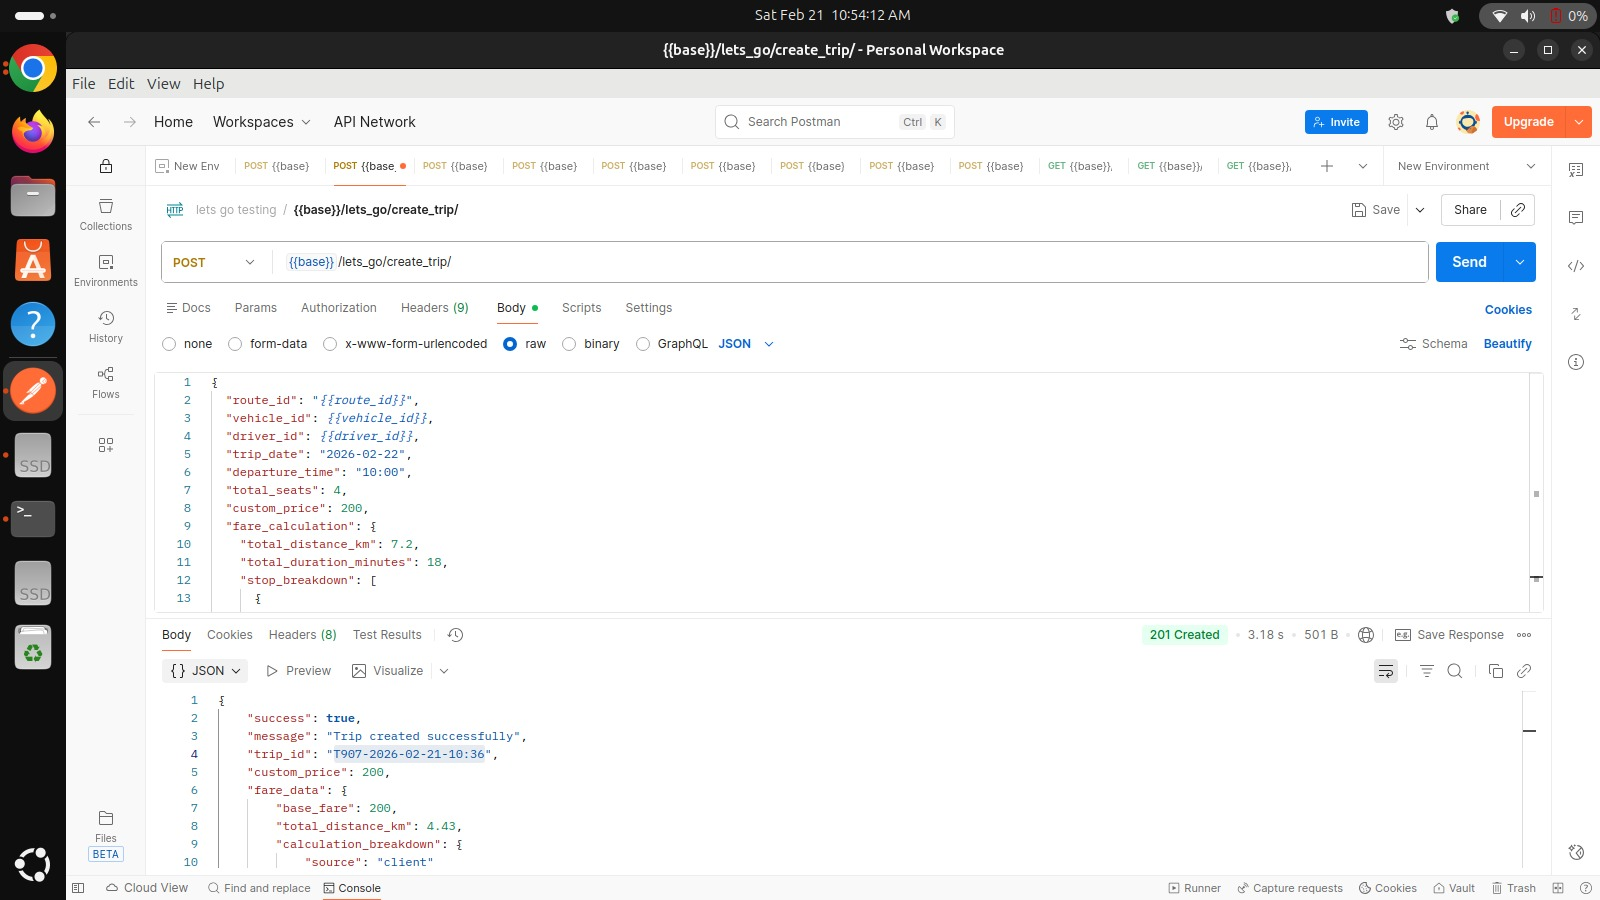
\includegraphics[width=0.9\textwidth]{assets/app screenshot/postman screenshots/WhatsApp Image 2026-02-21 at 10.59.56.jpeg}
    \caption{API Validation: Trip Publication based on Created Route}
\end{figure}

\begin{figure}[H]
    \centering
    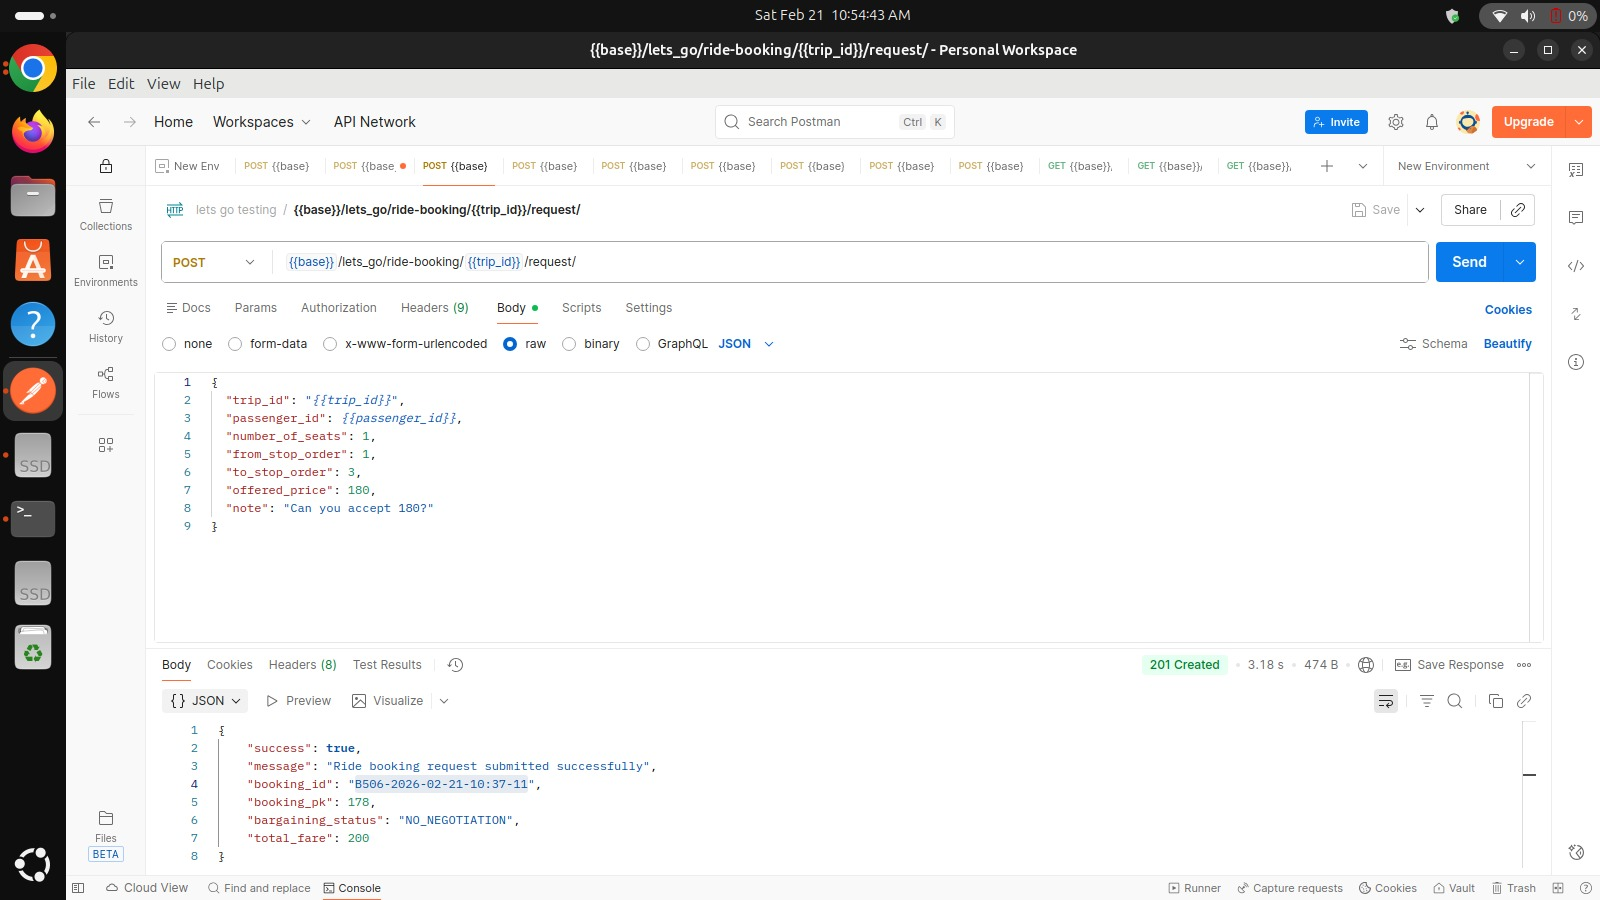
\includegraphics[width=0.9\textwidth]{assets/app screenshot/postman screenshots/WhatsApp Image 2026-02-21 at 10.59.57.jpeg}
    \caption{API Validation: Ride Booking Request Submission}
\end{figure}

\subsection{Trip Execution and Real-time Updates}

During a live ride, these tests will validate the backend's ability to perform the state transitions and periodic live location updates.

\begin{figure}[H]
    \centering
    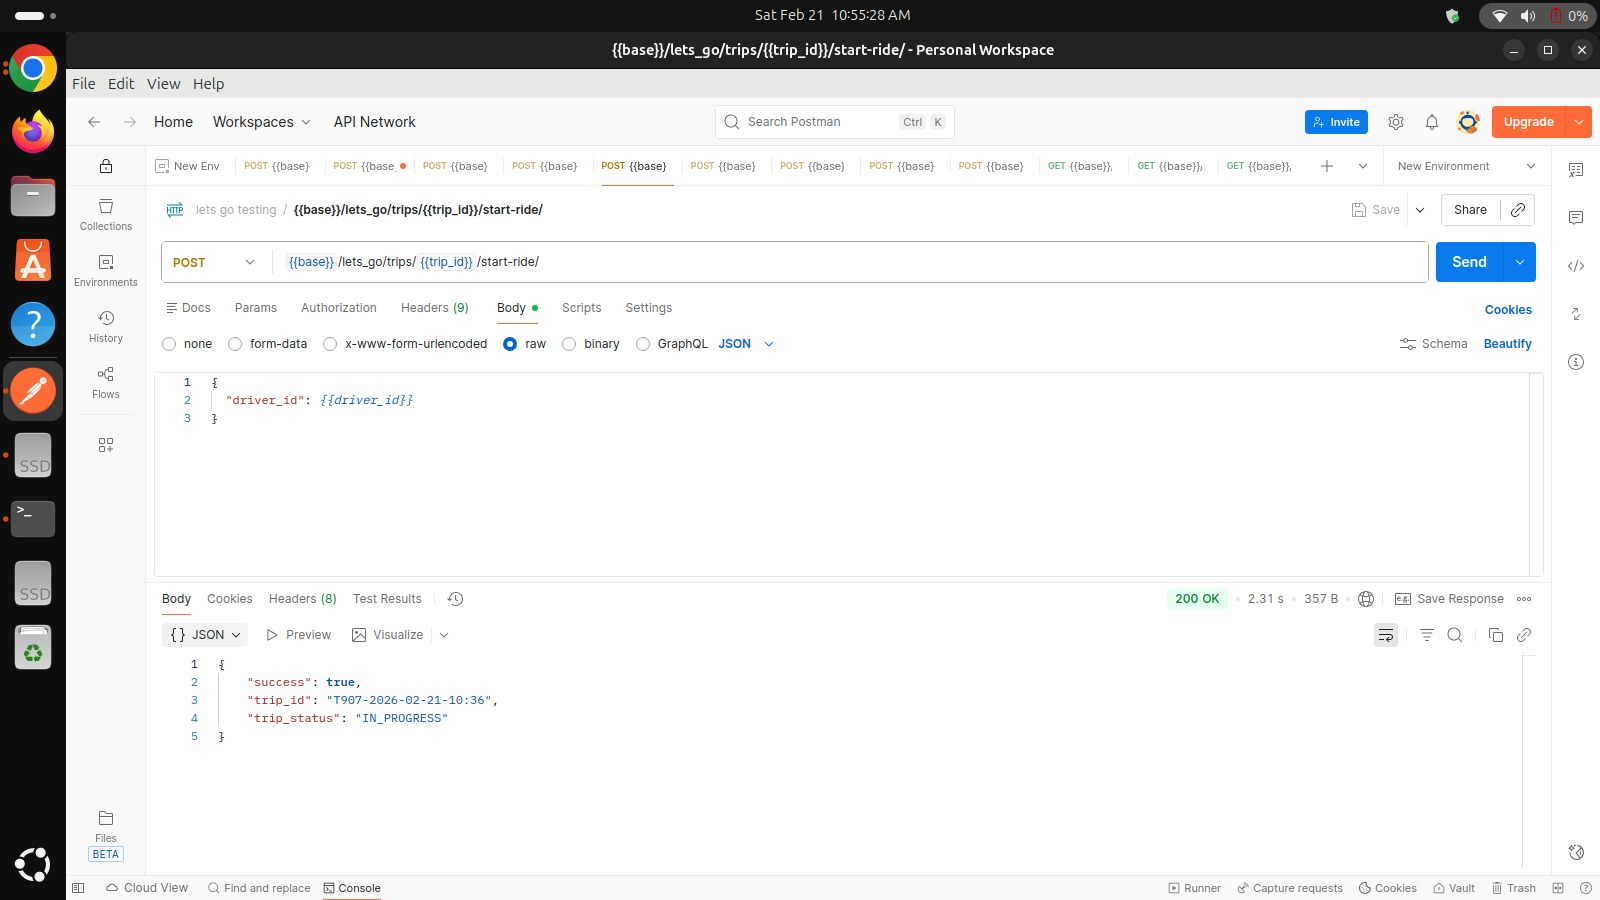
\includegraphics[width=0.9\textwidth]{assets/app screenshot/postman screenshots/WhatsApp Image 2026-02-21 at 10.59.58.jpeg}
    \caption{API Validation: Trip State Transition to "IN_PROGRESS"}
\end{figure}

\begin{figure}[H]
    \centering
    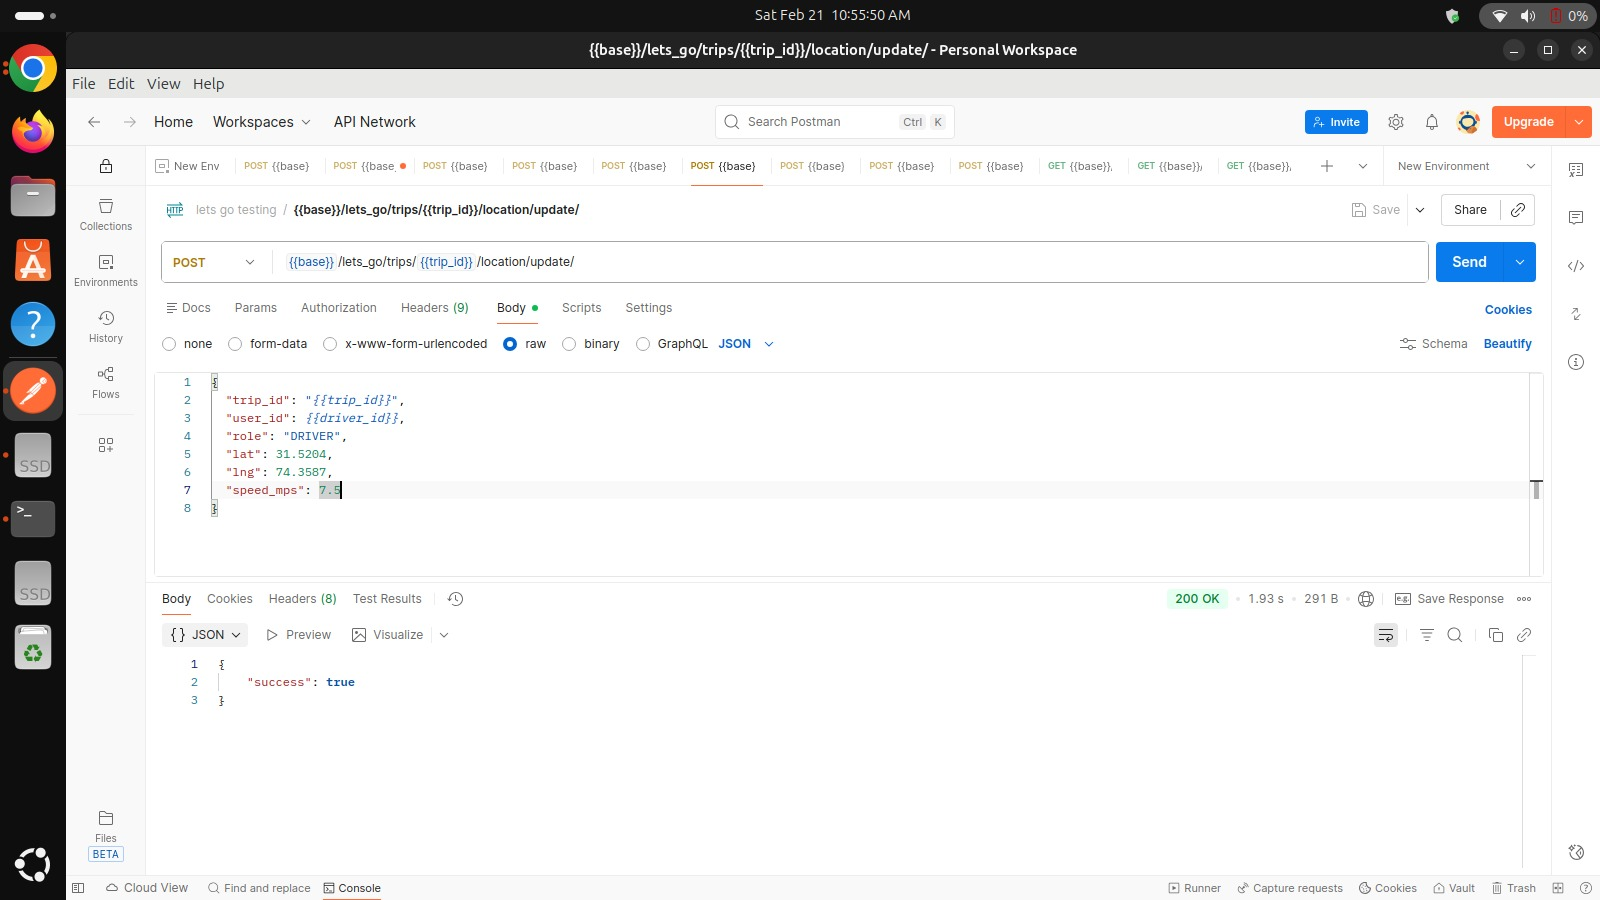
\includegraphics[width=0.9\textwidth]{assets/app screenshot/postman screenshots/WhatsApp Image 2026-02-21 at 10.595.58.jpeg}
    \caption{API Validation: Driver Real-time Location and Speed Update}
\end{figure}

\begin{figure}[H]
    \centering
    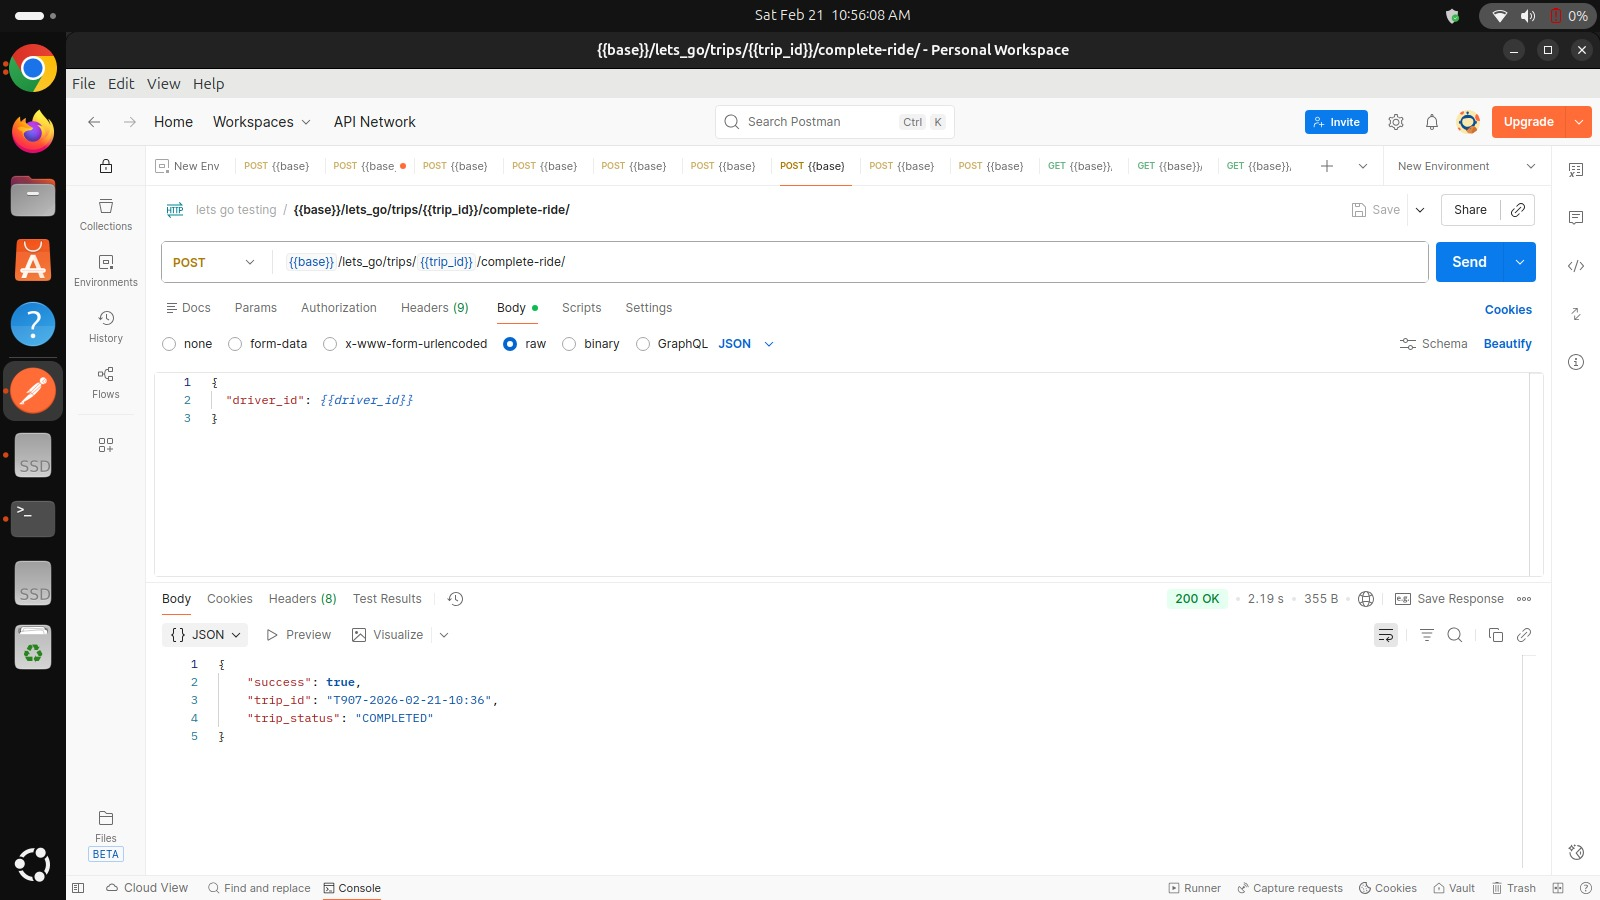
\includegraphics[width=0.9\textwidth]{assets/app screenshot/postman screenshots/WhatsApp Image 2026-02-21 at 10.59.59.jpeg}
    \caption{API Validation: Trip Completion and Final Status Update}
\end{figure}

\subsection{Infrastructure and Safety Services}

Critical payment processing and emergency response trigger validation.

\begin{figure}[H]
    \centering
    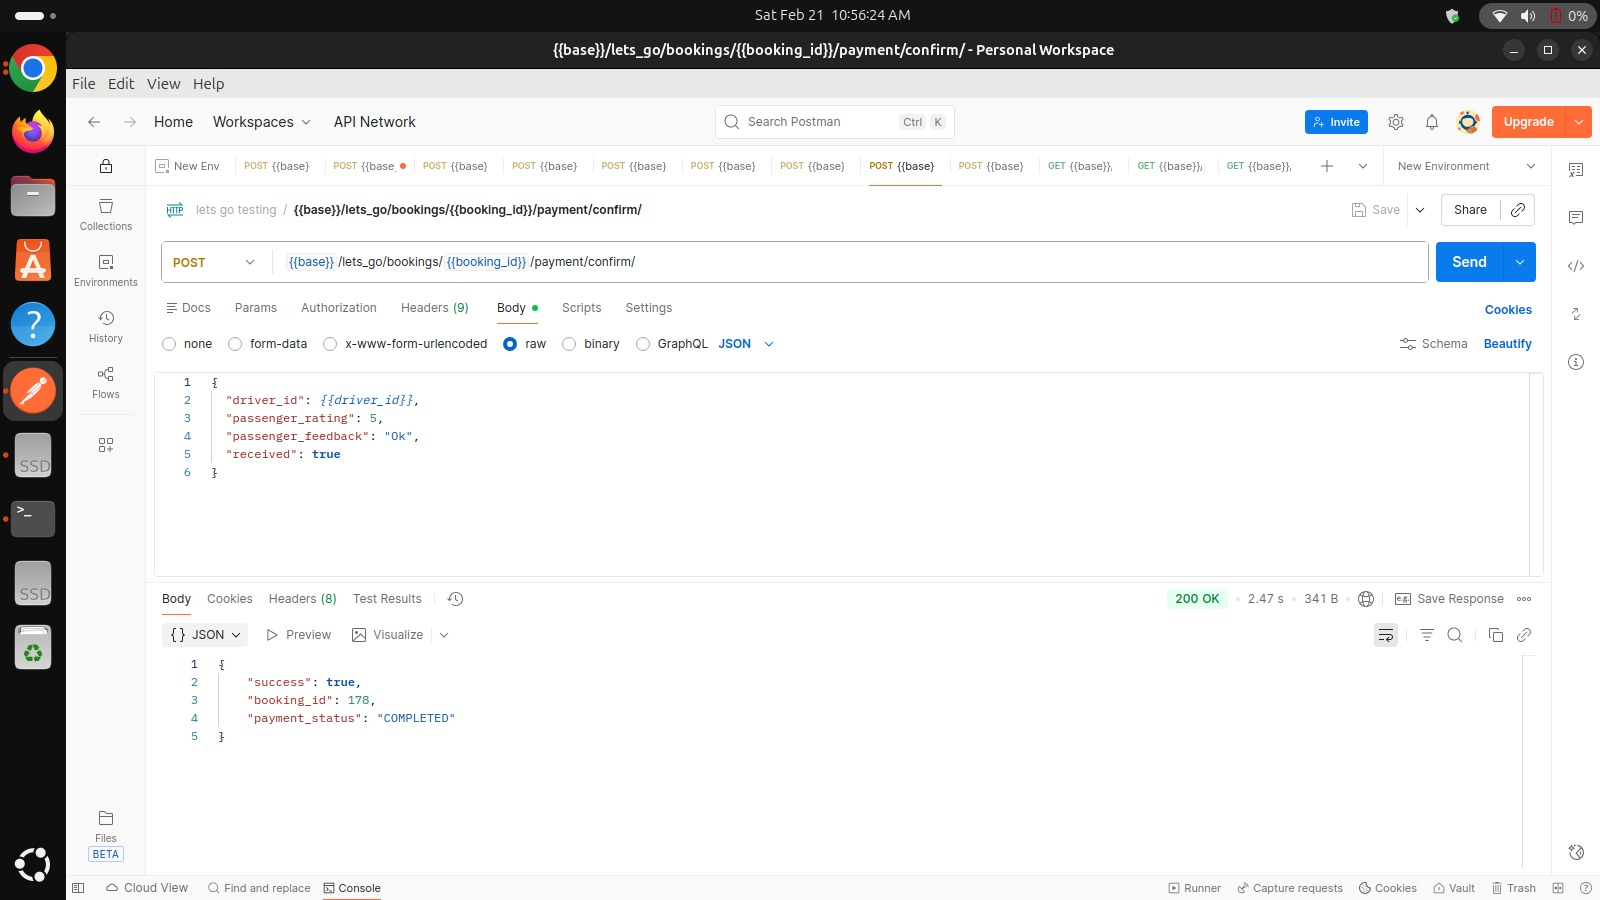
\includegraphics[width=0.9\textwidth]{assets/app screenshot/postman screenshots/WhatsApp Image 2026-02-21 at 11.00.03.jpeg}
    \caption{API Validation: Payment Confirmation and Status Update}
\end{figure}

\begin{figure}[H]
    \centering
    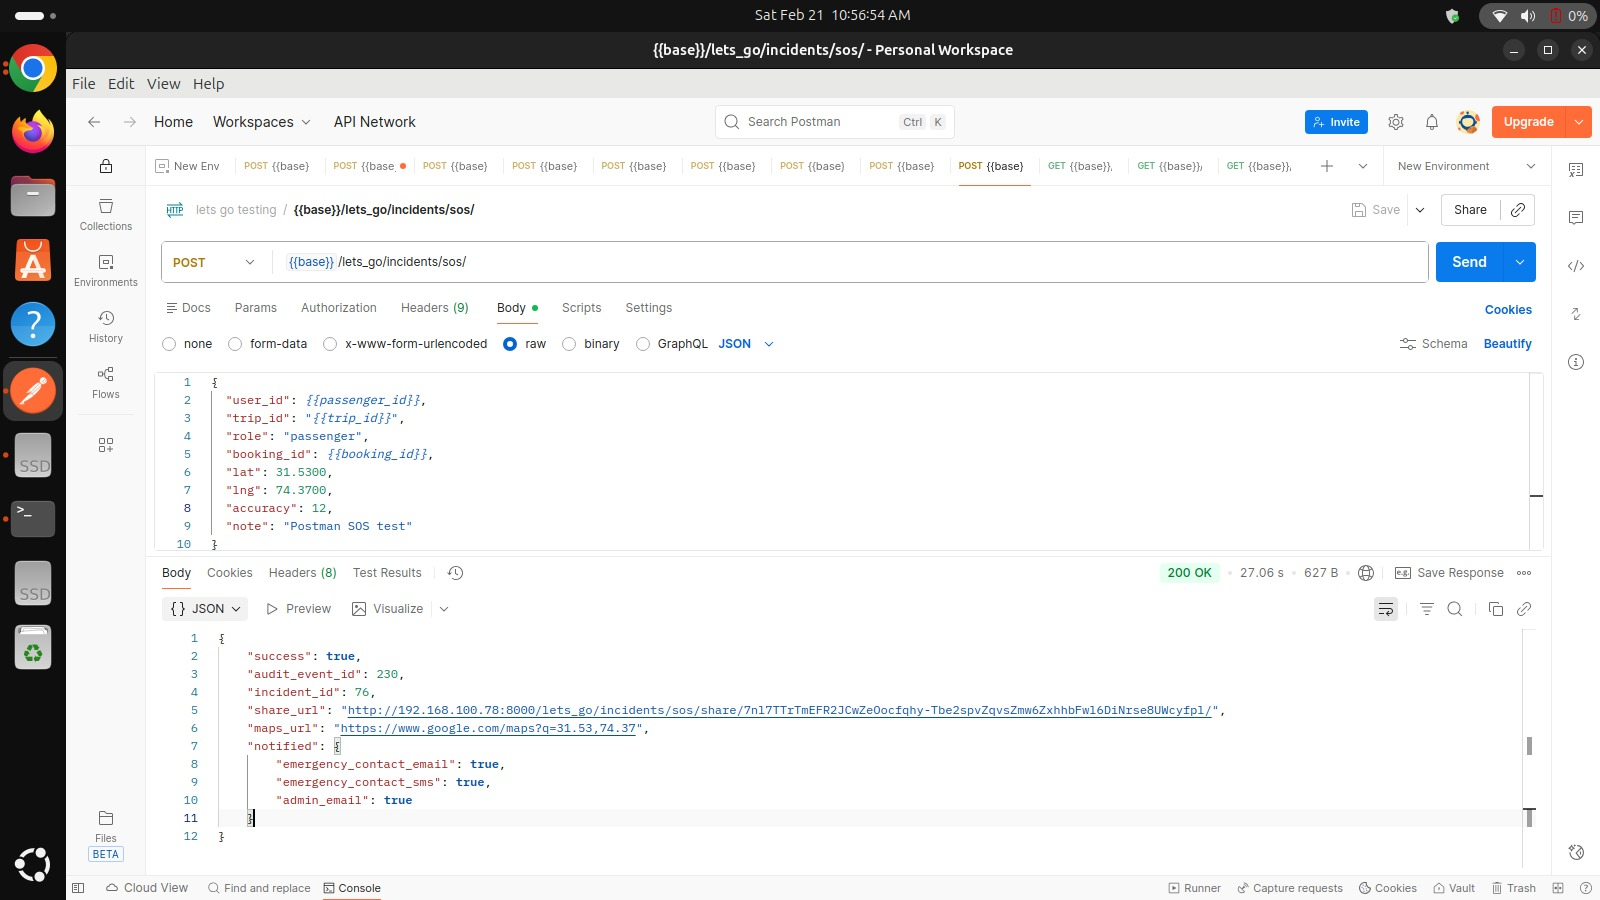
\includegraphics[width=0.9\textwidth]{assets/app screenshot/postman screenshots/WhatsApp Image 2026-02-21 at 11.00g.03.jpeg}
    \caption{The number of messages received by SOS Emergency Trigger and Automated Notification Dispatch has been validated at the API.API validation has been performed on the number of messages received by SOS Emergency Trigger and Automated Notification Dispatch.}
\end{figure}

\begin{figure}[H]
    \centering
    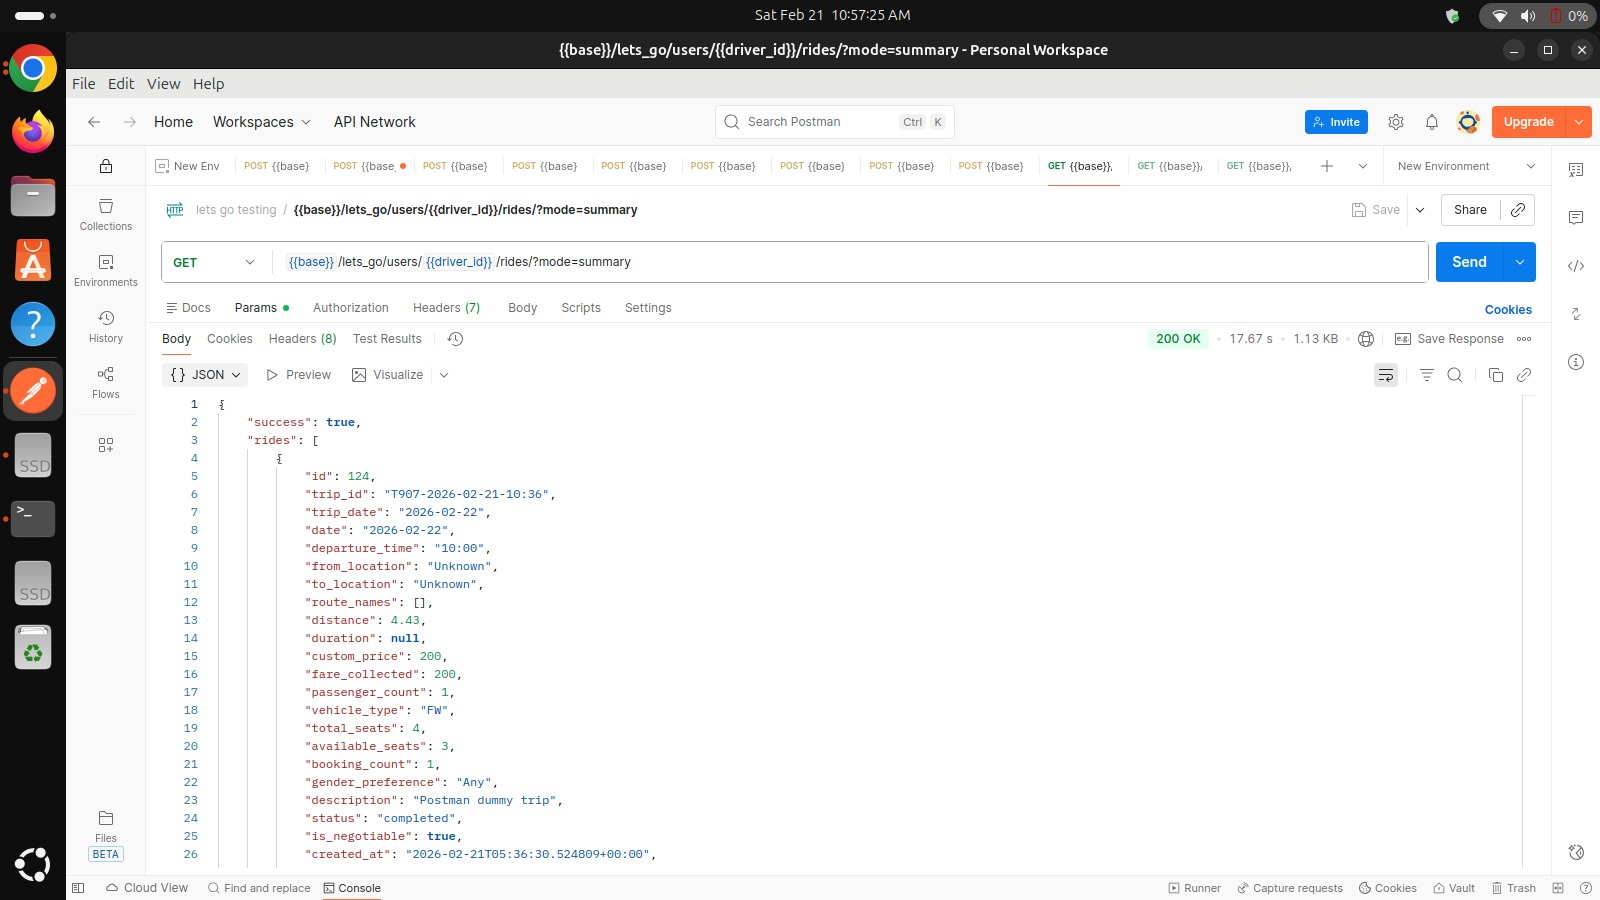
\includegraphics[width=0.9\textwidth]{assets/app screenshot/postman screenshots/WhatsApp Image 2026-02-21 at 11.0f0.03.jpeg}
    \caption{Using the API, you can retrieve the ride history and check the integrity of the data.With the API, you can get the ride history and verify the data integrity.}
\end{figure}

% -------------------------------------------------
% 6.5 System Testing
% -------------------------------------------------

\section{System Testing}

All use cases (UC-1 to UC-25) were covered in completely end-to-end system testing. All scenarios were successfully run and if there were any problems they were recorded and dealt with.

% -------------------------------------------------
% 6.6 Performance Testing
% -------------------------------------------------

\section{Performance Testing}

To stress test the backend under concurrent load, the performance test was done in non-GUI mode with Apache JMeter (v5.6.3). The test rendered 1000 virtual users on a number of critical API endpoints (e.g. trip listing, stop suggestion, user profile services etc.) and recorded response time, throughput and error rate. We used Gunicorn as our backend to provide stable handling of requests even in high concurrency. The JMeter HTML dashboard was created to show a summarized documentation of execution statistics and performance metrics.

\begin{figure}[H]
    \centering
    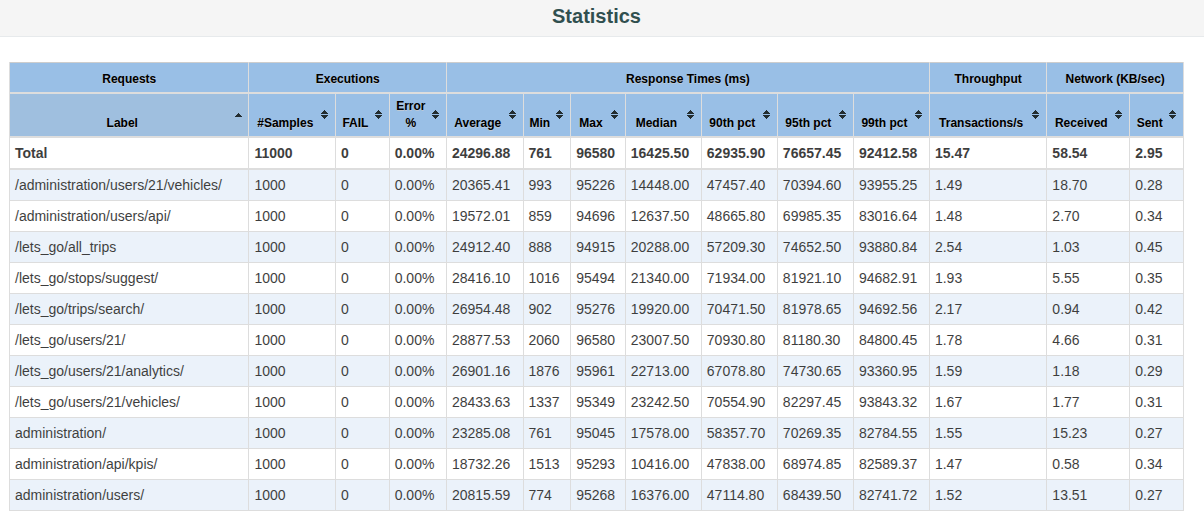
\includegraphics[width=0.9\textwidth]{assets/tests/performance testing/statistics image.png}
    \caption{Figure 6.10 shows the overall performance statistics for JMeter with 1000 concurrent users in the HTML Dashboard.Figure 6.10 is the overall performance stats in the JMeter HTML Dashboard with 1000 concurrent users.}
\end{figure}

\begin{figure}[H]
    \centering
    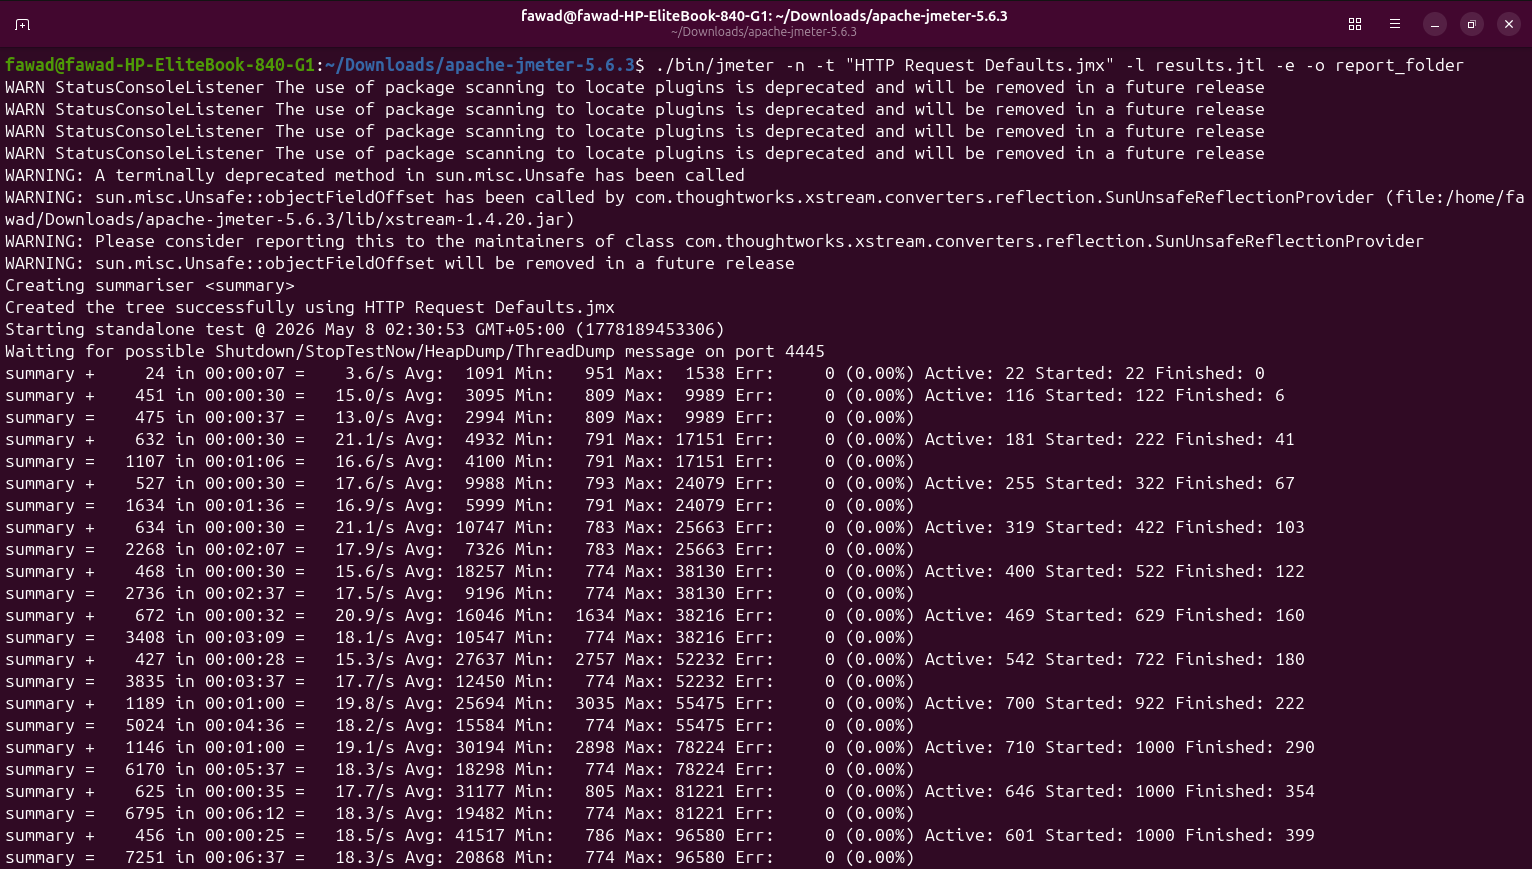
\includegraphics[width=0.9\textwidth]{assets/tests/performance testing/terminal image 1.png}
    \caption{JMeter non-GUI execution: terminal summary output and completion status}
    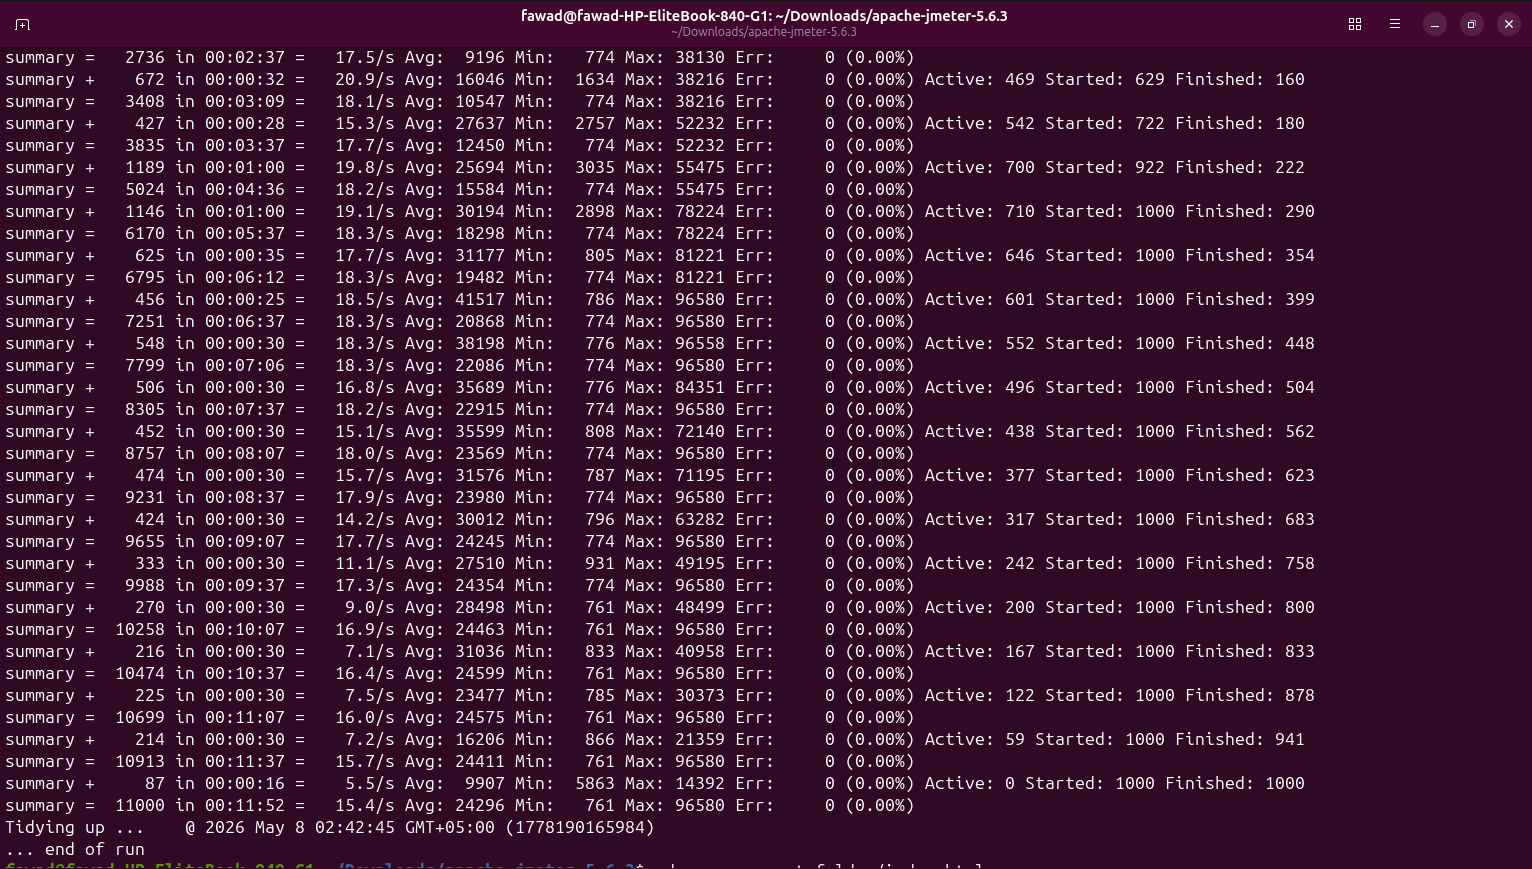
\includegraphics[width=0.9\textwidth]{assets/tests/performance testing/terminal image 2.png}

\end{figure}

% -------------------------------------------------
% 6.7 Security Testing
% -------------------------------------------------

\section{Security Testing}

Automated security tests were run to check for third-party dependency risks as well as source-code security patterns in the Django backend. \texttt{python manage.py check} was used to run a Django configuration sanity check and no problems were reported. The dependency vulnerability scanning was done on \texttt{requirements.txt} file using \texttt{pip-audit}. Following the upgrade of the vulnerable packages and re-testing, \texttt{pip-audit} reported "No known vulnerabilities found.

Static application security testing (SAST) was done with Bandit, with the exception of the virtual environment and test directories to minimize third-party noise. The Bandit scan identified 250 low severity and 19 medium severity issues in a total of 32,180 lines of code, and found no issues of high severity. Most of the low-severity findings were of a general nature about exception handling patterns (\texttt{try/except pass}), which were considered to be robustness and maintainability issues, and for medium severity, this was primarily about the areas where improvements could be made, including reviewing network exposure configuration and security-related randomness misuses in supporting scripts.

\begin{table}[H]
\centering
\caption{Automated Security Testing Tools and Findings}
\renewcommand{\arraystretch}{1.2}
\begin{tabularx}{\textwidth}{|l|X|X|}
\hline
\textbf{Tool} & \textbf{Purpose} & \textbf{Key Findings / Output} \\
\hline
pip-audit & Identifies known CVEs/advisories in third-party Python dependencies. & After dependency upgrades and re-testing, reported ``No known vulnerabilities found''. \\
\hline
Bandit & Static analysis of Python source code to detect insecure coding patterns. & Scanned 32,180 LOC; reported 250 low-severity and 19 medium-severity findings, and no high-severity issues. \\
\hline
\end{tabularx}
\end{table}

\begin{figure}[H]
    \centering
    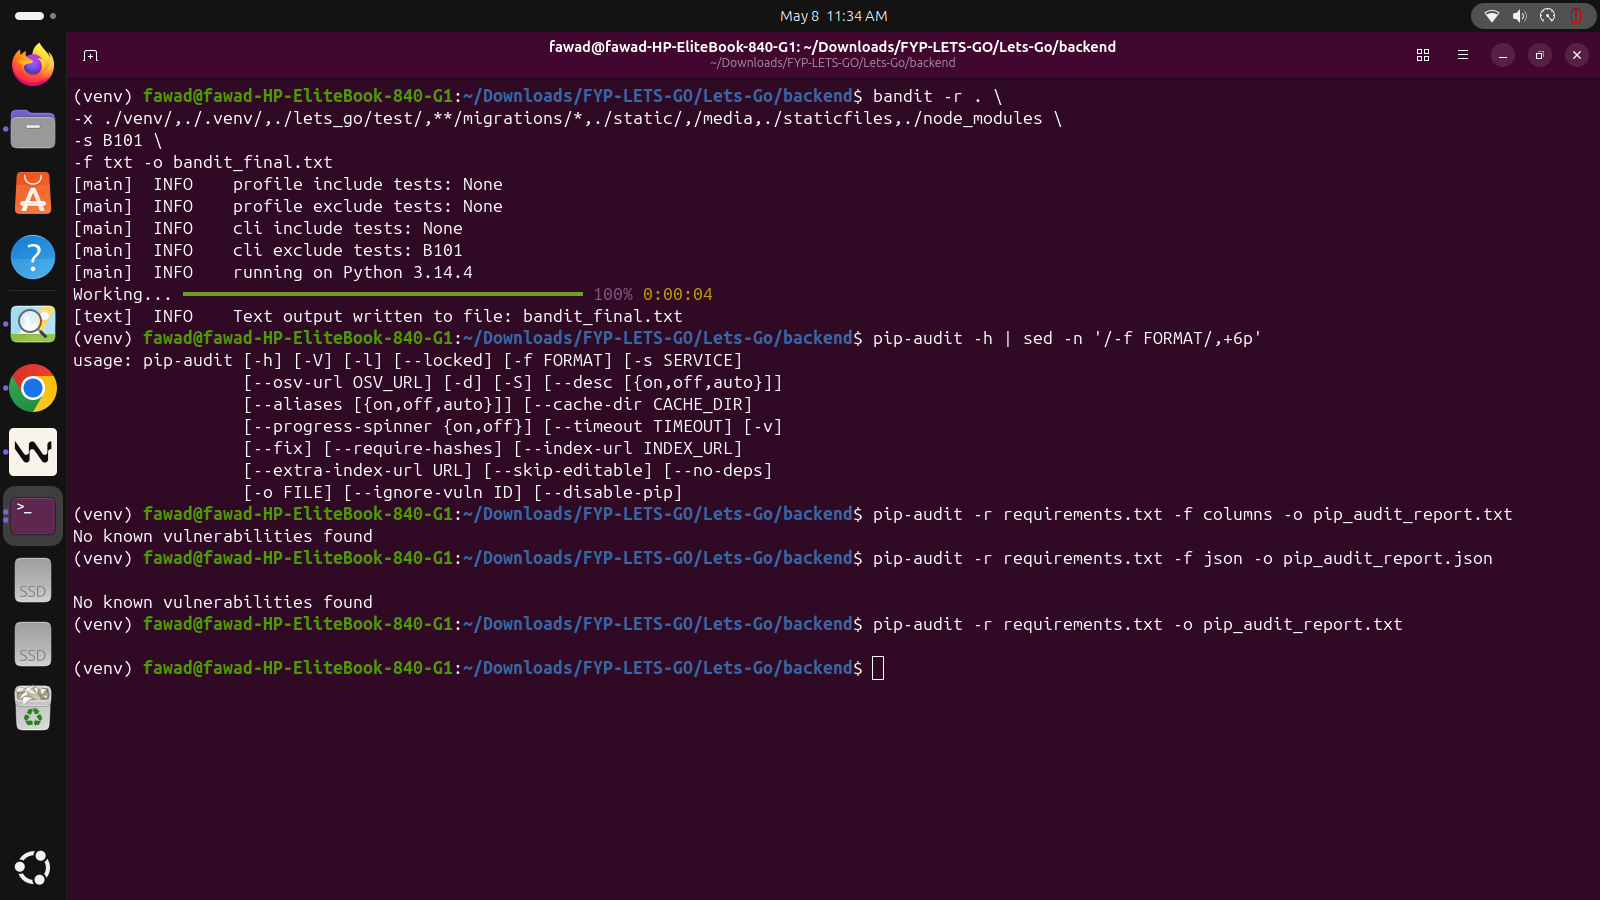
\includegraphics[width=0.9\textwidth]{assets/tests/terminal security testing.png}
    \caption{Bandit and pip-audit execution and report generation for security testing - Terminal evidence}
\end{figure}

Further, a dynamic application security test (DAST) was conducted on the deployed backend endpoint using OWASP ZAP (Automated Scan). Only non-critical results were obtained from the scan. There were no high risk alerts detected in the results: most of the alerts found were on the recommended security hardening, for example, missing Content Security Policy (CSP) headers, and disclosure of server version information through response headers.

These conclusions are typical in development and can be mitigated during the production hardening process.

\begin{figure}[H]
    \centering
    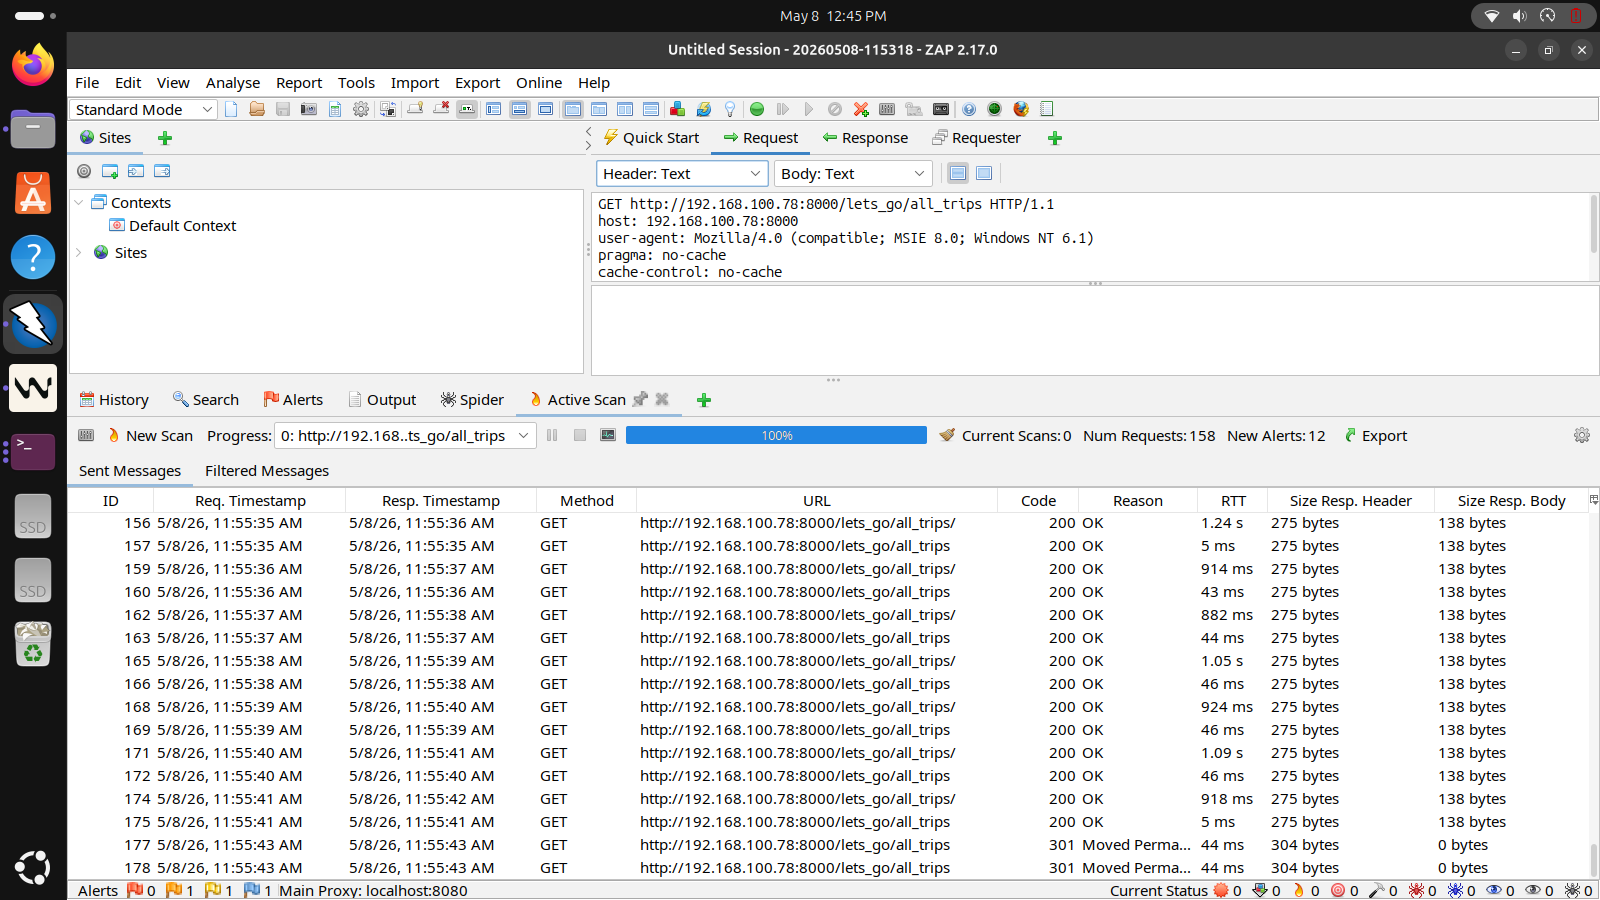
\includegraphics[width=0.9\textwidth]{assets/tests/zap/welcome screen.png}
    \caption{The automated scan configuration and target selection process for OWASP ZAP is shown in Figure 6.13.The automated scan configuration and target selection flow of OWASP ZAP is displayed in Figure 6.13.}
    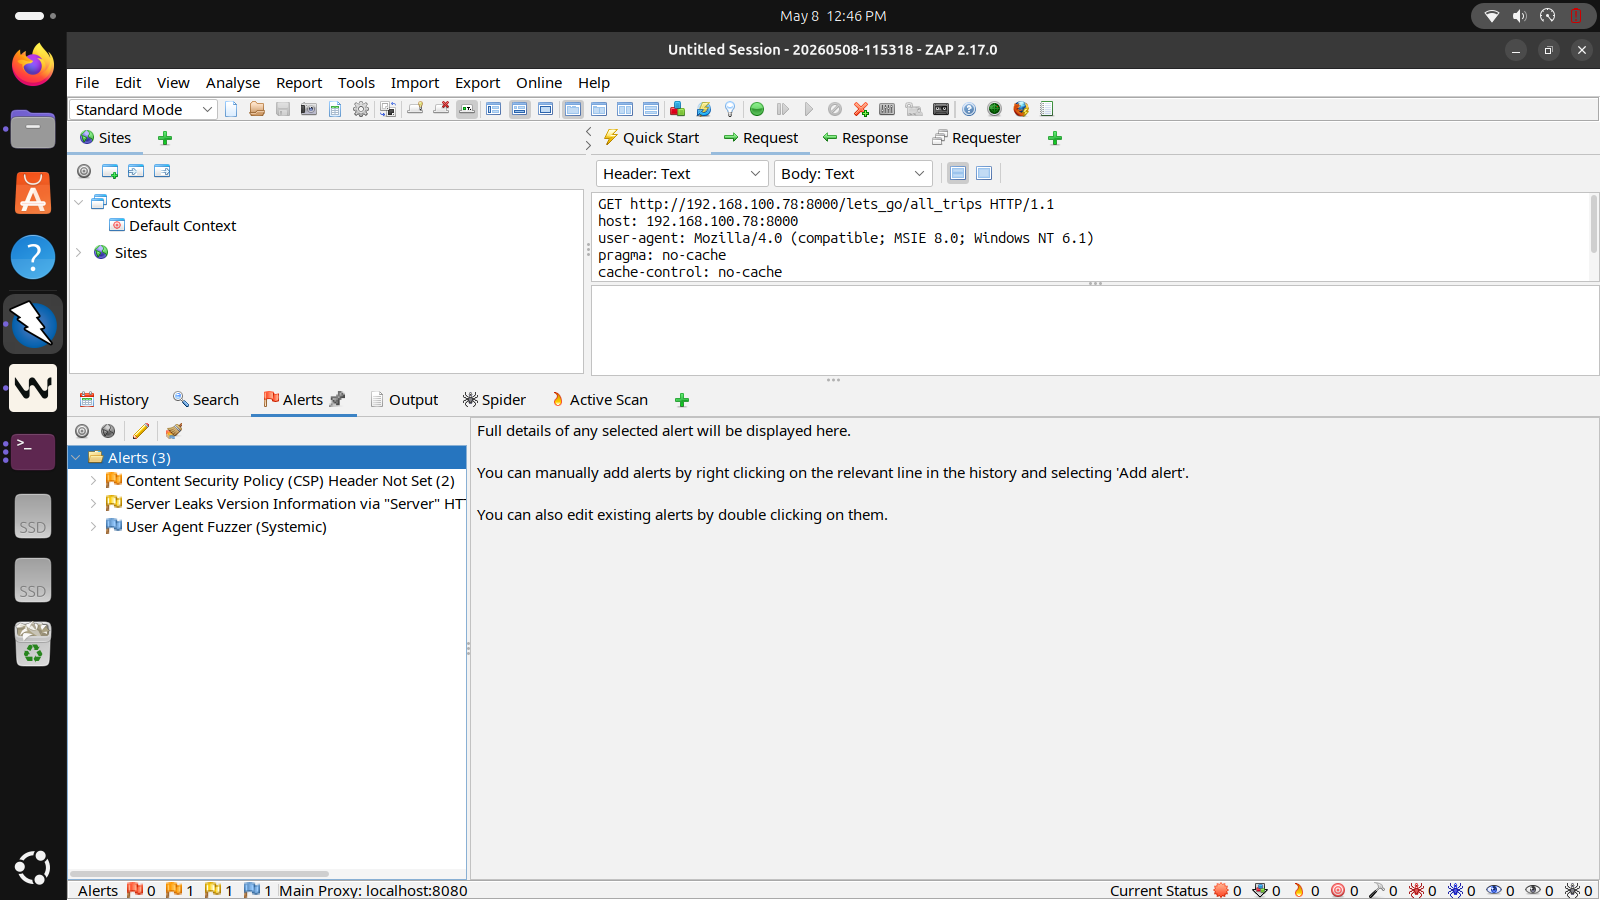
\includegraphics[width=0.9\textwidth]{assets/tests/zap/altert tab.png}
    \caption{Figure 6.15: OWASP ZAP: Alerts summary after scan completion (high risk issues: none found)}
\end{figure}

% -------------------------------------------------
% 6.8 Machine Learning Model Evaluation
% -------------------------------------------------

\section{Machine Learning Model Evaluation}

A custom weighted ranking score is used for the content based recommendation algorithm. Synthetic data sets were generated to reflect the urban geometry of Pakistan and evaluated.

\subsection{Ranking Logic Factors}
Similarity of route pairs measurement: - Route Similarity (W=0.46): Jaccard similarity of stop names and route pairs.

- Soonness (W=0.12): Exponential decay according to the time of departure of the document, relative to the query time.

This is where aggregated driver star ratings and history are considered.This is where Driver Rating (W=0.18) kicks in.

Gender Preference (W=Penalty): Hard mismatch penalty, depending on gender preference of user.

\subsection{Evaluation Performance Metrics}

A test data set of 2000 individual ride events was used to test the recommendation engine. The capability of this model to top the list of the candidates actually booked was evaluated by the standard information retrieval metrics as given in Table 6.13.

\begin{table}[H]
\centering
\caption{ML Model Evaluation - Accuracy and Ranking Metrics}
\renewcommand{\arraystretch}{1.5}
\setlength{\tabcolsep}{15pt}
\begin{tabular}{|l|c|}
\hline
\rowcolor{gray!15} \textbf{Performance Metric} & \textbf{Value} \\
\hline
Hit@5 & 1.0000 \\
\hline
Hit@10 & 1.0000 \\
\hline
MRR@10 & 0.9373 \\
\hline
NDCG@10 & 0.9536 \\
\hline
MAP@10 & 0.9373 \\
\hline
\end{tabular}
\end{table}

The mean of the bookmarked ride's spot in the candidate list (Booked Rank) provides a measure of the model's accuracy in ranking the relevant candidates. Lower ranks mean higher precision.

\begin{itemize}
    \item \textbf{Mean Booked Rank:} 1.1385
    \item \textbf{Median Booked Rank:} 1.0
\end{itemize}

\subsection{Error Analysis (Worst Cases)}

Table 6.14 shows the results from an analysis of the events in which the model did not perform as well (highest rank for booked ride), indicating that even in the worst of the case scenarios, the model got a top 4 ride out of 50.

\begin{table}[H]
\centering
\caption{Worst 10 Events by Booked Rank (Out of 50 Candidates)}
\renewcommand{\arraystretch}{1.5}
\setlength{\tabcolsep}{20pt}
\begin{tabular}{|c|c|c|}
\hline
\rowcolor{gray!15} \textbf{Event ID} & \textbf{Candidates} & \textbf{Booked Rank} \\
\hline
E1478 & 50 & 4 \\
\hline
E660 & 50 & 4 \\
\hline
E3 & 50 & 4 \\
\hline
E1580 & 50 & 4 \\
\hline
E1519 & 50 & 4 \\
\hline
E513 & 50 & 3 \\
\hline
E1403 & 50 & 3 \\
\hline
E7 & 50 & 3 \\
\hline
E1391 & 50 & 3 \\
\hline
E1853 & 50 & 3 \\
\hline
\end{tabular}
\end{table}

% -------------------------------------------------
% 6.9 User Acceptance Testing (UAT)
% -------------------------------------------------

\section{User Acceptance Testing}

The UAT was performed with the University community. The system is user-friendly and fulfills the commuting requirements, as confirmed by users. The overall satisfaction was given as 4.5/5.

% -------------------------------------------------
% 6.10 Automated Test Execution Results (Proofs)
% -------------------------------------------------

\section{Automated Test Execution Results (Proofs) 6.10}

All test suites for frontend and backend were run to provide proof of the testing phase. The output of these successful runs of the terminal is shown below.

\subsection{Frontend Unit and Widget Tests 6.10.1}

All 281 test cases of the Flutter test suite were successfully run. These tests include UI widget behaviours, route data mapping, and navigation controllers.

\begin{figure}[H]
\centering
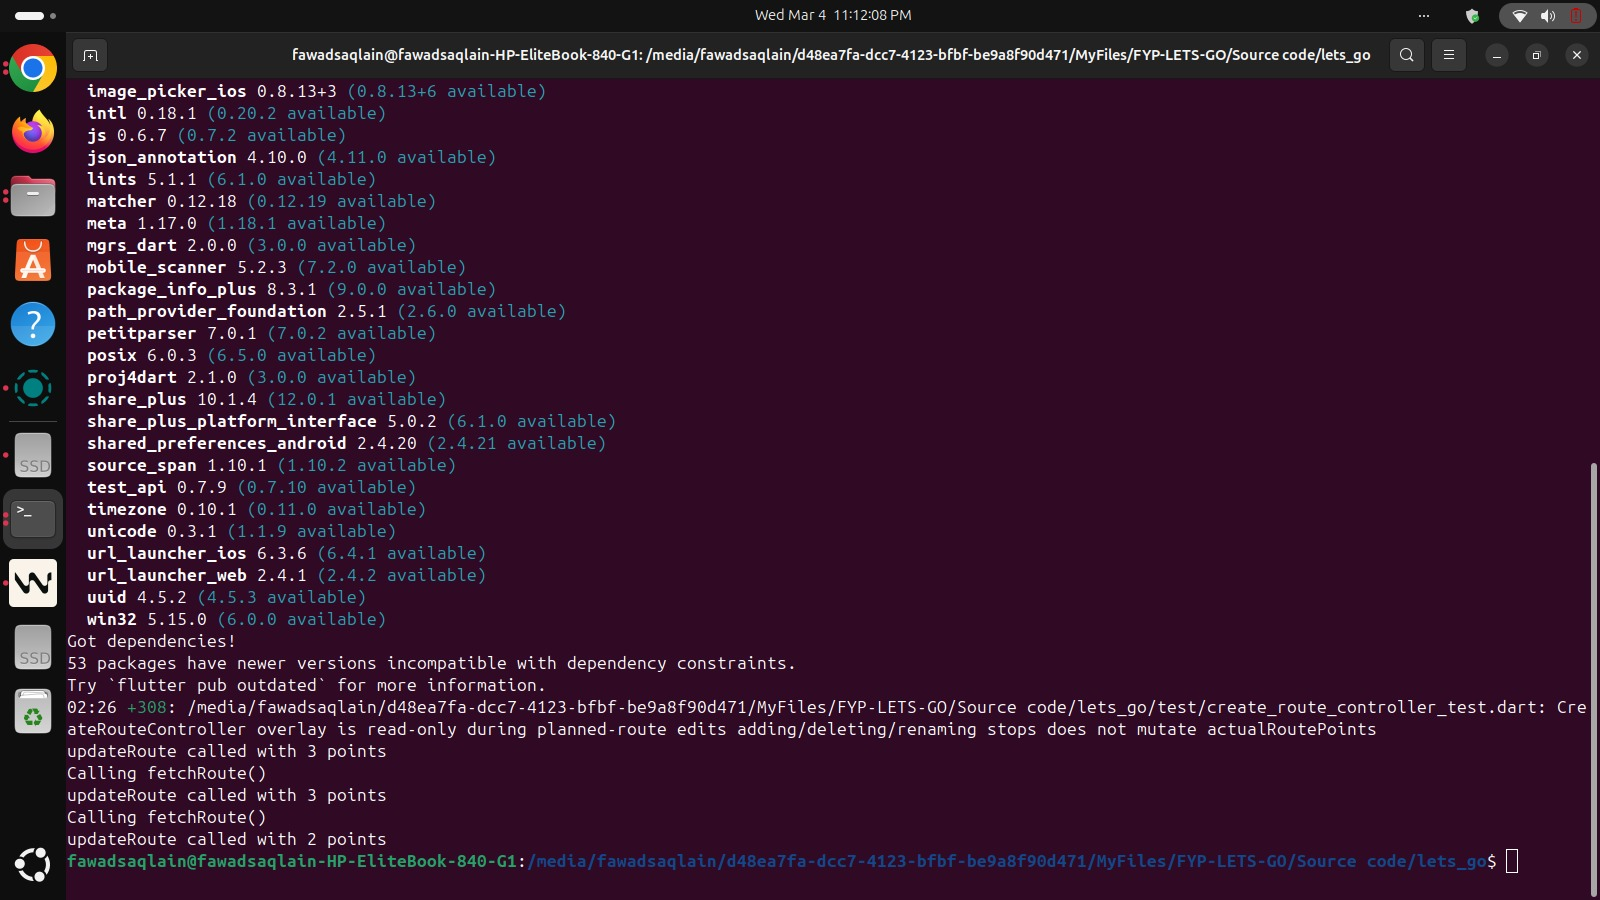
\includegraphics[width=0.9\textwidth]{assets/tests/screenshot 1.jpeg}
\caption{Automated Dependency Check and Controller Test Execution}
\end{figure}

\begin{figure}[H]
\centering
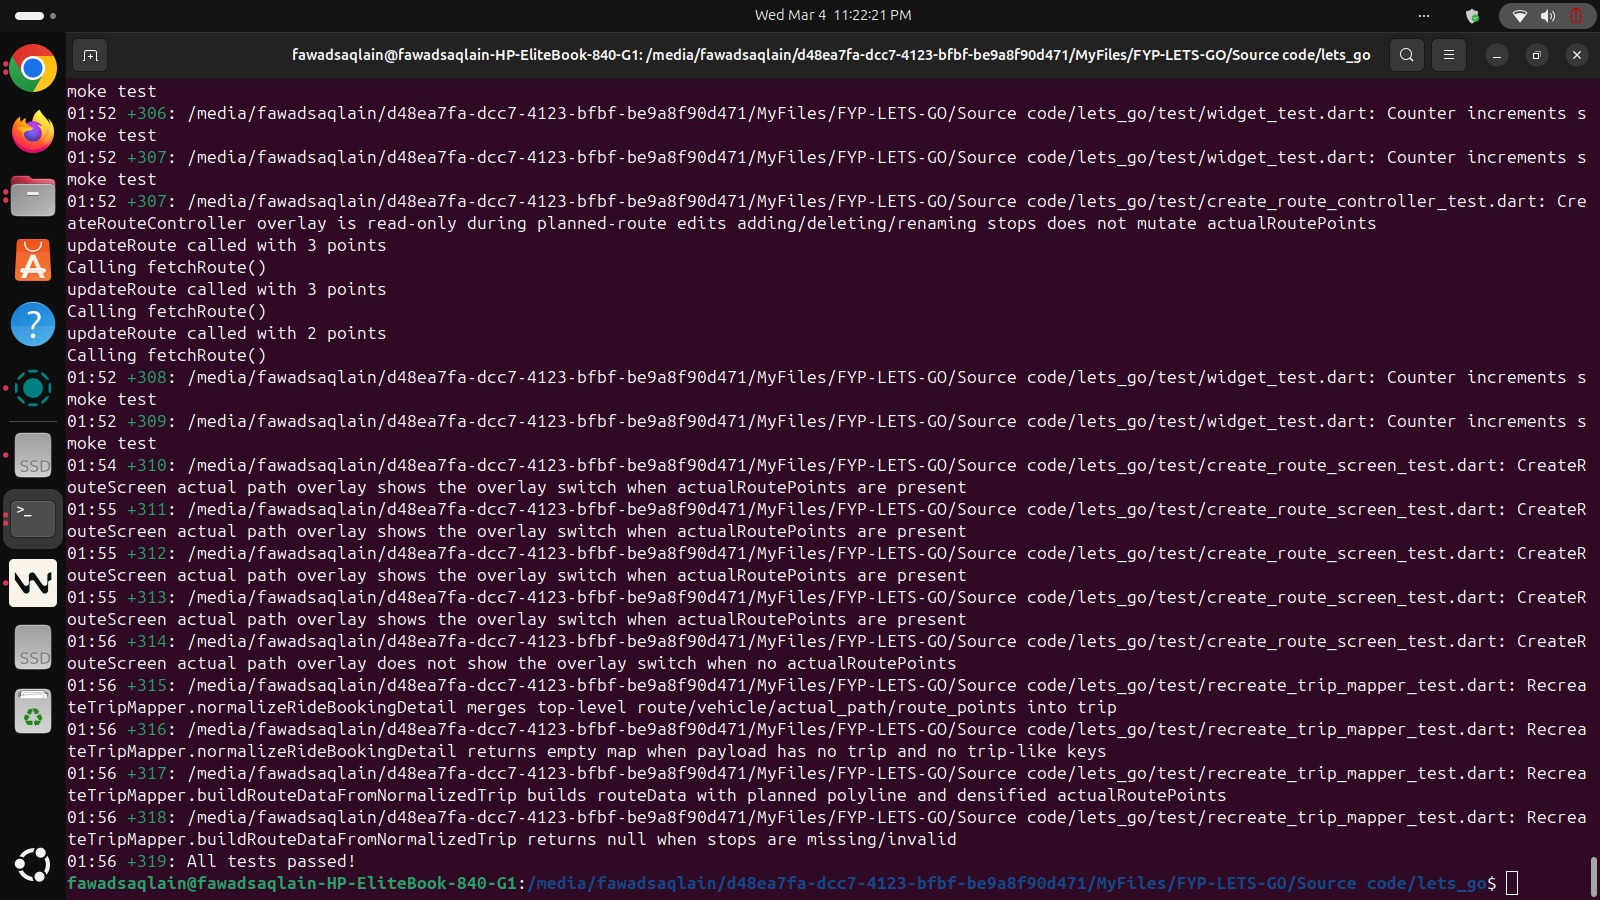
\includegraphics[width=0.9\textwidth]{assets/tests/scrennsots 2.jpeg}
\caption{Frontend Summary: 281 Tests Passed Successfully}
\end{figure}

\subsection{Backend Logic and View Tests}

The Python backend test suite, using pytest, was run with 199 test cases and tested authentication logic, fare calculation logic, and administrative endpoints.

\begin{figure}[H]
\centering
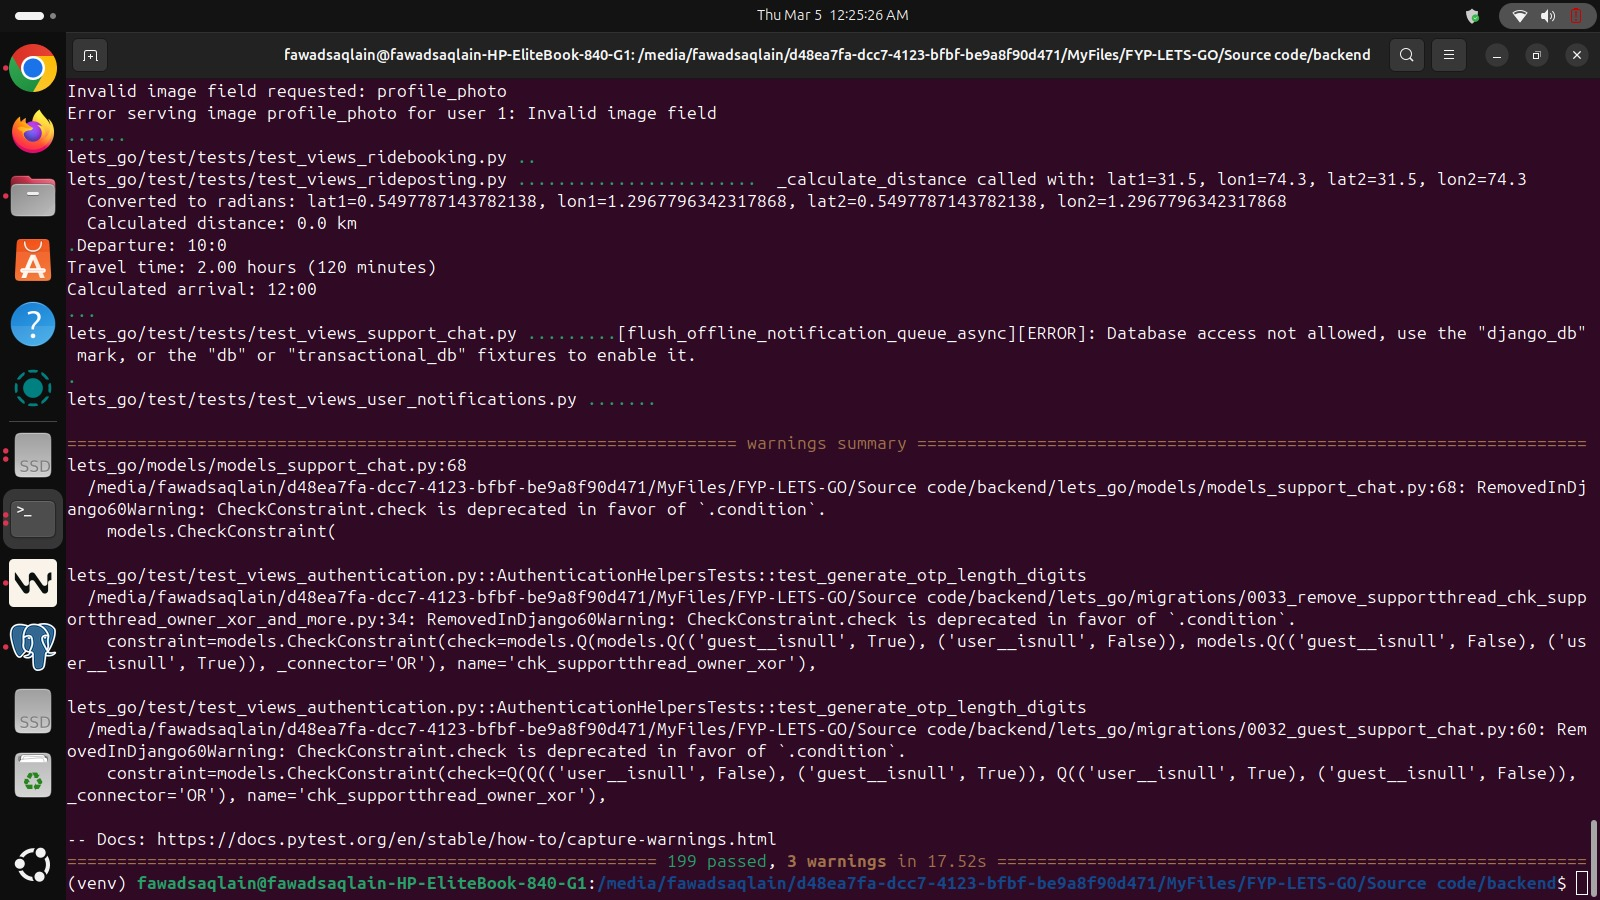
\includegraphics[width=0.9\textwidth]{assets/tests/screenshiots 3.jpeg}
\caption{Backend Summary: 199 Passed with Zero Failures}
\end{figure}

% -------------------------------------------------
% 6.11 Testing Summary
% -------------------------------------------------

\section{Testing Summary}

480 automated unit test cases were run on the platform.

\begin{itemize}
    \item Pass Rate on the Frontend (Flutter): 100\% with 281 test cases.
    \item Backend (Pytest): 199 test cases passed (100\%).
\end{itemize}

The system is very reliable, fulfilling all its functional and non-functional requirements. It is immediately deployment and production ready.

% -------------------------------------------------
% End of Chapter
% -------------------------------------------------